\chapter{Introduction}
\label{introduction}
Current internet architecture is mostly based on TCP/IP stack, which allows establishing communication channels between two IP addresses. While it worked great for past years, it struggles to fit current demands. Today the internet is dominated by transporting content such as audio, video, images, and text from content creators to content consumers. 

% Write more about how the internet is used today
% Write more about why current architecture doesn't fit 
% ICN - the solution !!!
The Information-centric networks introduce a paradigm shift from a host-centric to a content-oriented paradigm. Placing content in the center of interest. This allows us to achieve several benefits. All network participants become more aware of the transferring content. This kind of awareness allows implementing various improvements over host-based paradigms such as content caching, mobility, integrity, and security assurance. All of those features are guaranteed naively by the ICN transport layer in contrast to TCP/IP where we needed to build them on top of it. 

Many projects are implementing the ICN approach: Data-Oriented Network Architecture (DONA), Named Data Networking (NDN), Publish-Subscribe Network Technology (PURSUIT), Scalable and Adaptable Network Solutions (SAIL), Inter-planetary File System (IPFS).

They all differ in details, but the core concepts are the same, they try to achieve a communication model that is suited for disconnections, disruptions, mobility, and transferring large data to a large number of devices. They introduce the in-network storage on each node for data caching. They also decouple senders from receivers, by resolving content by its name---not the location of the host. 
In ICN data is requested by its name (Named Data Object - NDO), and is served by the closest possible node who is holding it. That allows efficient caching on the transport layer---relieving the application layer from implementing a cache strategy individually. 

When we write NDO, we understand any arbitrary data that can be transferred over the network: web page, music, images, video, documents, and data streams. What's most important NDOs compared to traditional URLs are location independent, they do not specify the location where the content should be served from, nor how they should be transferred to the receiver. NDO granularity may differ from packets to data chunks to whole data objects, depending on the approach and data size.

Data naming is the most significant concept in ICN. Data names must be unique––similarly to hostnames in current Internet architecture; two different DNS nodes should resolve one domain name to the same location––two different ICN nodes must resolve one name to the same content. 
There are two approaches to a naming system: hierarchical - similar to URL, and flat - global namespace, often just the hash of the file.
Additionally, each NDO should be authenticated with the publisher who created it. Digital signatures on data objects guarantee both integrity and authentication. If the data is trusted, not the host, then the data can be served from any untrusted source––and we still can trust it.

\section{Named Data Networking}
To get better understanding of how ICN networks work, we describe one of the most mature project–––Named Data Networking (NDN). The design was initialy proposed under the name Content-Centric Network by Van Jacobson in 2006 \cite{4ANewWay38:online}. Currently the project is under development with name Named Data Networking \cite{NamedDat22:online}. 

NDN replace TCP/IP protocol stack by placing the chunks of named content in place of IP addresses (see Fig \ref{fig:ndn-design}a). The only layer that can not be changed is the layer 3–––the thin "waist" of the stack. All protocols in rest of the layers can be adjusted to the needs.
\begin{figure}[h!]
  \subfloat[]{
	\begin{minipage}[c][1\width]{
	   0.5\textwidth}
	   \centering
	   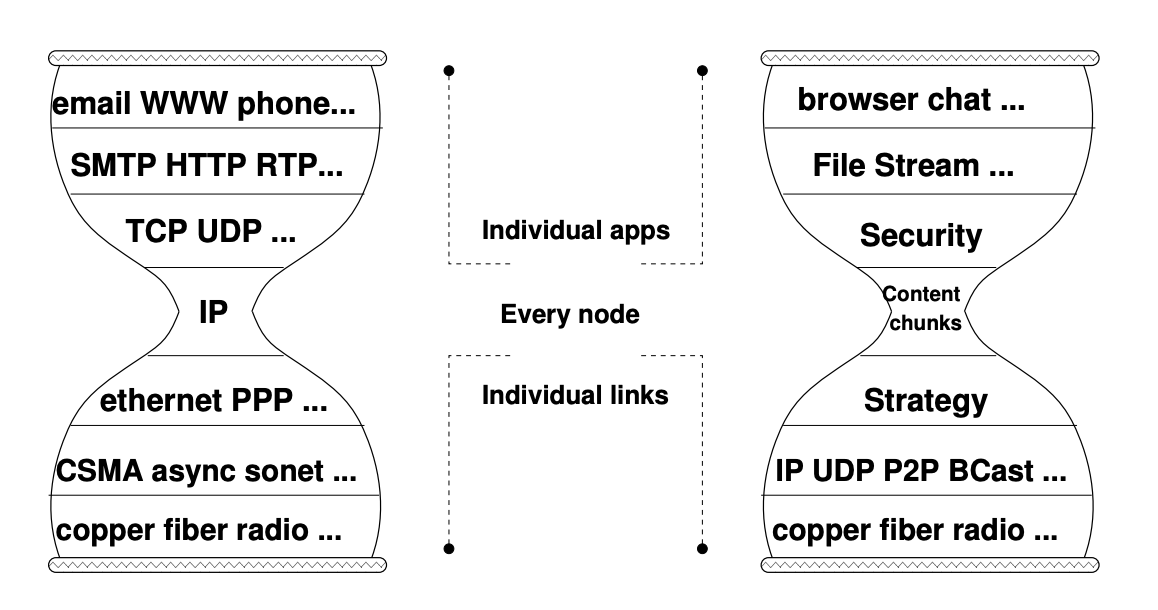
\includegraphics[height=0.5\textwidth]{img/ndn-stack.png}
	\end{minipage}}
 \hfill 	
  \subfloat[]{
	\begin{minipage}[c][1\width]{
	   0.5\textwidth}
	   \centering
	   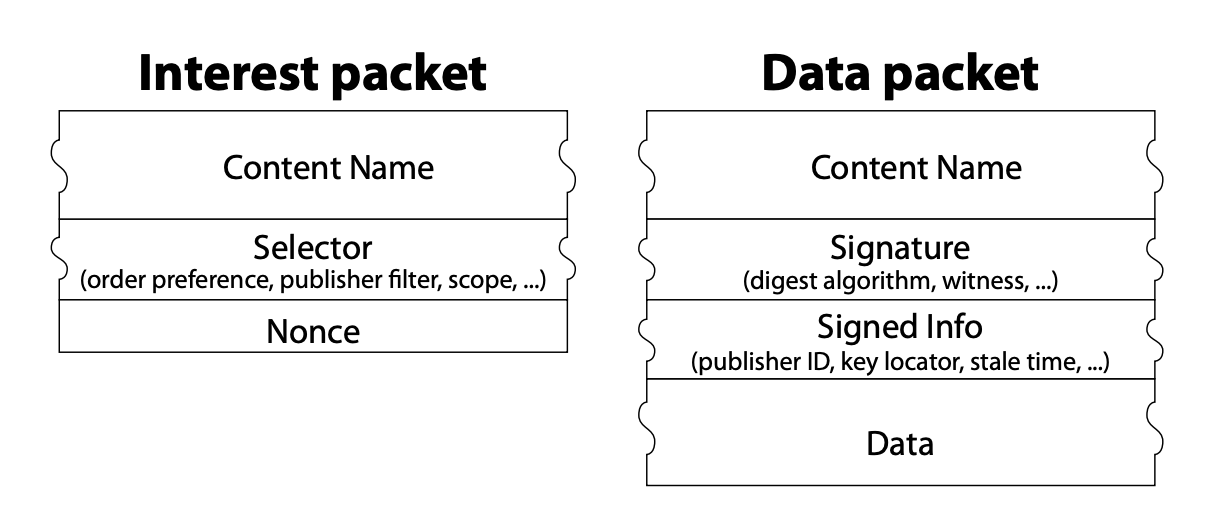
\includegraphics[height=0.5\textwidth]{img/ndn-packets.png}
	\end{minipage}}
\caption{Named Data Networking design. Source \cite{jacobson2009networking}}
\label{fig:ndn-design}
\end{figure}
NDN defines two types of packets: Interest, and Data (see Fig. \ref{fig:ndn-design}b). Interest packet as the name suggest, indicate the interest of some data chunk, where the data chunk is identified by its Content Name. An consumer broadcast a Interest packet to all its connection faces. If any node that receive such message has the corresponding data locally (in Content Store), it can respond with the Data Packet, otherwise the Interest is forwarded to next router..
The operations of NDN node are similar to IP node. In Fig. \ref{fig:ndn-operations} we can see the forward engine model in NDN node. When request arrive at one of the available faces it get dispatched based on the lookup result. 

The FIB (Forwarding 
Information Base) is responsible for forwarding the interests to potential nodes where the data can be found (similar to FIB used in IP, except it allows for multiple outgoing faces rather than single one). 

The Content Store(CS) is responsible for buffering a content that was requested by Interest packet. Since the data can be served to multiple consumers–––not just single connection, as it is done in IP––it is not recycled after the first Interest request is satisfied. This mechanism is called in-network storage, because the network itself is storing the data. It is possible due to idempotency, self-identification, and self-authentication of the packets so each packet is equally useful for many consumers (e.g. two hosts interesting in Netflix video, can receive the content from single node without requesting the Netflix servers). The data is stored as long as possible and different storage policy can be used e.g. LRU replacement.

The PIT (Pending Interest Table) store information about the interests forwarded to potential data sources. When one of them reply with the Data packet, the PIT is checked if some consumer is waiting for the data, and if so, the Data packet is forwarded to corresponding face.
\begin{figure}[h]
    \centering
    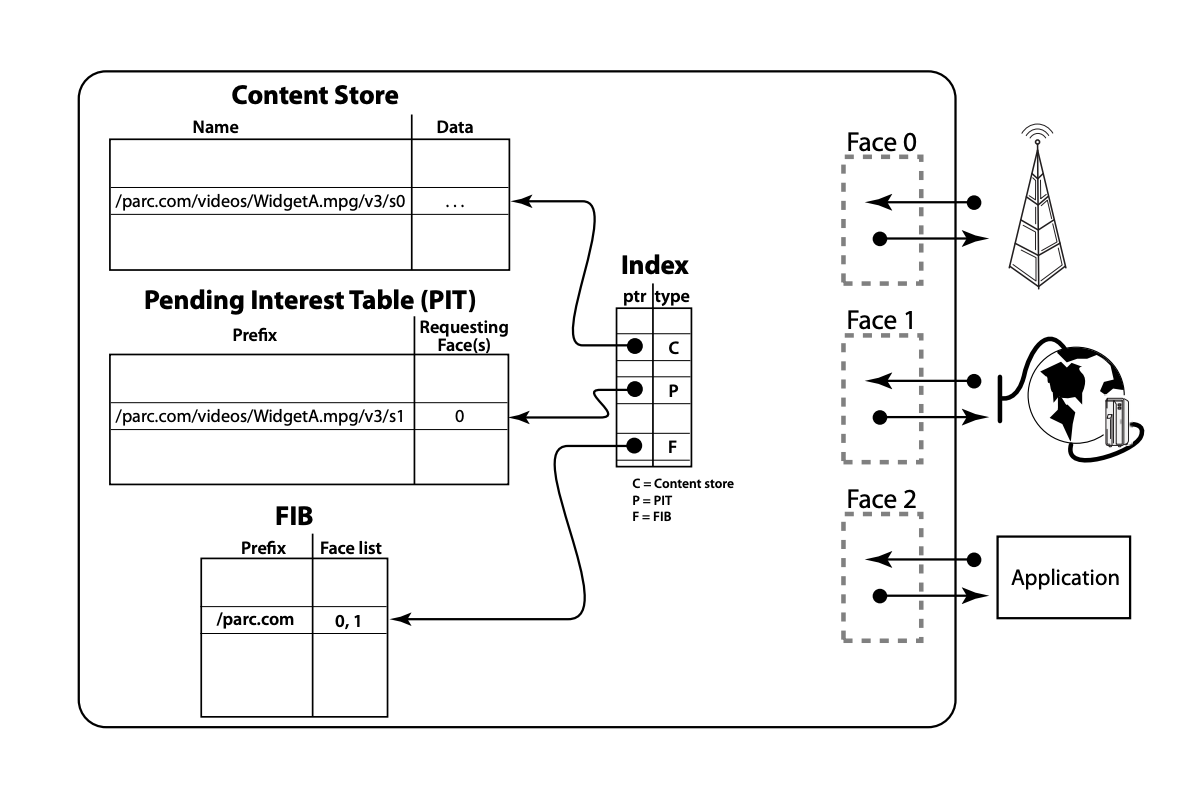
\includegraphics[width=\linewidth]{img/ndn-operations.png}
    \caption{NDN node operations. Source \cite{jacobson2009networking}}
    \label{fig:ndn-operations}
\end{figure}

To better understand the model, the concrete packet flow is presented in Fig.\ref{fig:ndn-flow}. 
\begin{enumerate}
    \item 1. The requester application wants to receive some data so it sends the request to its local NDN engine. The node first check the local CS, and since the concent is absent, it request the Interest packet to the closes router.
    \item 2. The router first check its Content Store, and if the data is absent, it check if there is already pending interest in PIT for such data, if not the request is forwarded to the next router according to FIB.  
    \item 3. The next router do the same as previous router, it check its CS, PIT, and then forward the Interest packet through FIB.
    \item 4. Finally the Interest reaches the data source router, where the content is present in the CS so it is immediately returned.
    \item 5. The router receive the Data packet and store it in its CS, check which nodes are waiting for the data in PIT and forward the Data packet accordingly.
    \item 6. This router (that was initialy requested by the requestor) do the same as the previous router storing the data in CS and responding with the Data packet.
    \item After some time, different requestor send the Interest packet to its closest router.
    \item Router lookup the Content Name and finds out that the content is already stored in CS, therefore it immediately return the Data packet–––saving the network bandwidth and reducing the latency.
\end{enumerate}

\begin{figure}[h]
    \centering
    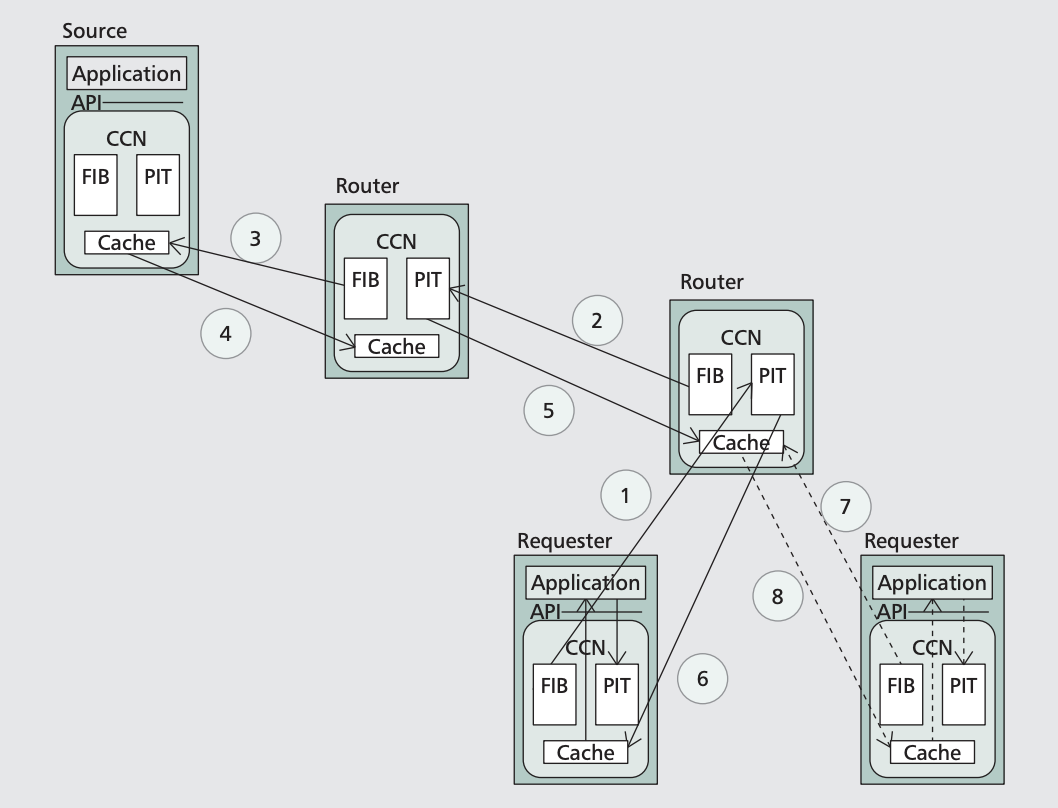
\includegraphics[width=\linewidth]{img/ndn-flow.png}
    \caption{NDN packets flow. Source \cite{ahlgren2012survey}}
    \label{fig:ndn-flow}
\end{figure}

%\section{IPFS}
%IPFS (Inter-planetary file system)\cite{benet2014ipfs} is a peer-to-peer distributed file system; its goal is to create a global file system where each file is indexed by its content hash. 
%In the traditional web, we request file by its URI - which then resolves to a certain location where the content is hosted. In IPFS we request a file by its content hash - which then resolves to the closest location where the file can be accessed; it can be either: cache, local storage, our neighbor, our ISP node, any other peer in the network, or finally the content publisher. This is possible not because of the structure of the network, but because we request the content. In the traditional web, each time we request the URI it can resolve to different content, therefore we can not trust our neighbor, that he will send us the content we were asking for. 
%Additionally, in IPFS, each content is signed by its publisher keypair, so we can be sure that the content that our neighbor is serving us, is the thing that was created by the publisher. Therefore if we request a malicious link (hash of the content) and it's integral with its content, we still can reject it -- if it's not signed by the actual publisher we are interested in. 
%We can state that IPFS natively guarantees integrity and authentication.

%The fact that the content is authenticated by the publisher keypair seems to be perfectly fine. But here in this thesis, we double down on possible threats and propose solutions on how to solve them.
